% DO NOT COMPILE THIS FILE DIRECTLY!
% This is included by the other .tex files.

\begin{frame}[t,plain]
\titlepage
\end{frame}

\begin{frame}
    \frametitle{\texttt{\$ whoarewe}}
    \begin{center}
        
\includegraphics[width=0.8\linewidth]{pictures/whoarewe.png}
    \end{center}
    \vspace*{0.5em}
    \begin{center}
        \frame{
\includegraphics[width=0.24\linewidth]{pictures/belgian-joke}}
    \end{center}
\end{frame}

\begin{frame}
    \frametitle{Automation in MISP: What already exists?}
    
\includegraphics[valign=m,width=16px]{pictures/python-logo.png}\hspace*{0.5em} \textbf{MISP API / PyMISP}
    \hspace*{0.25em}
    \begin{itemize}
        \item Needs CRON Jobs in place
        \item Potentially heavy for the server
        \item Not realtime
    \end{itemize}
    \vspace*{1em}
    
\includegraphics[valign=m,width=16px]{pictures/zeromq.png}\hspace*{0.5em} \textbf{PubSub channels}
    \hspace*{0.25em}
    \begin{itemize}
        \item After the actions happen: No feedback to MISP
        \item Tougher to put in place \& to share
        \item Full integration amounts to develop a new tool
    \end{itemize}
    \vspace*{0.5em}
    $\rightarrow$ No way to \textbf{prevent} behavior\\
    $\rightarrow$ Difficult to setup \textbf{hooks} to execute callbacks
\end{frame}

\begin{frame}
    \frametitle{What type of use-cases are we trying to support?}
    \begin{itemize}
        \item \textbf{Prevent} default MISP behaviors to happen
        \begin{itemize}
            \item Prevent \textbf{publication of events} not passing sanity checks
            \item Prevent \textbf{querying} thrid-party \textbf{services} with sensitive information
            \item $\cdots$
        \end{itemize}
        \vspace*{1.0em}
        \item \textbf{Hook} specific actions to run callbacks
        \begin{itemize}
            \item \textbf{Automatically run} enrichment services
            \item Modify data on-the-fly: False positives, enable CTI-Pipeline
            \item Send notifications in a chat rooms
            \item $\cdots$
        \end{itemize}
    \end{itemize}
\end{frame}

\begin{frame}
    \frametitle{Simple automation in MISP made easy}
    \begin{center}
        
\includegraphics[width=0.3\linewidth]{pictures/automation.png}
    \end{center}
    \begin{itemize}
        \item Why?
        \begin{itemize}
            \item Everyone loves \textbf{simple automation}
            \item \textbf{Visual} dataflow programming
            \item Users want \textbf{more control}
        \end{itemize}
        \item How?
        \begin{itemize}
            \item \textbf{Drag \& Drop} editor
            \item Prevent actions \textbf{before they happen}
            \item Flexible \textbf{Plug \& Play} system
            \item \textbf{Share} workflows, \textbf{debug} and \textbf{replay}
        \end{itemize}
    \end{itemize}
\end{frame}

\begin{frame}
    \frametitle{Content of the presentation}
    \begin{itemize}
        \item MISP Workflows fundamentals
        \item Demo with examples
        \item Using the system
        \item How it can be extended
    \end{itemize}

    \vspace*{1em}
    \begin{center}
        \frame{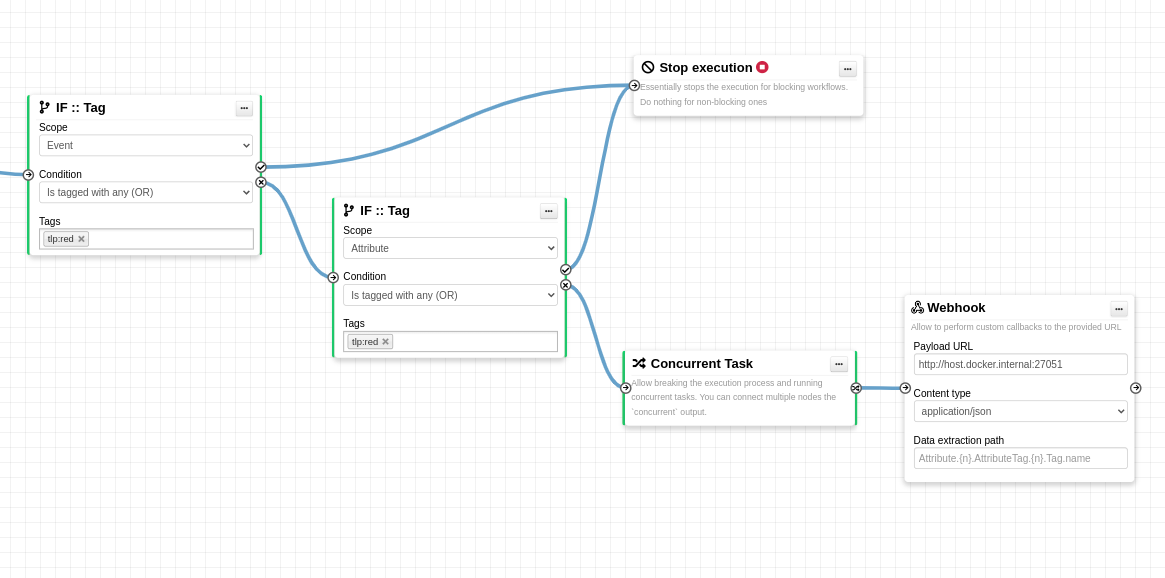
\includegraphics[width=0.7\linewidth]{pictures/overview.png}}
    \end{center}
\end{frame}

% \section{Workflow - Fundamentals}
\begin{frame}
    \frametitle{
        \huge
        \linebreak
        \linebreak
        \linebreak
        Workflow - Fundamentals
        \vspace{1em}
    }
    \textbf{Objective:} Start with the foundation to understand the basics
    \begin{center}
        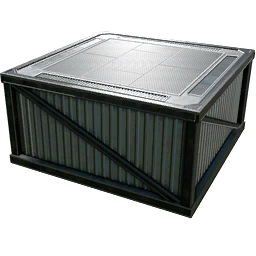
\includegraphics[width=0.07\linewidth]{pictures/fundation}
    \end{center}
\end{frame}


\begin{frame}
    \frametitle{How does it work}
    \begin{center}
        \frame{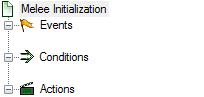
\includegraphics[width=0.6\linewidth]{pictures/event-condition-action.png}}
    \end{center}
    \begin{enumerate}
        \item An \textbf{event} happens in MISP
        \item Check if all \textbf{conditions} are satisfied
        \item Execute all \textbf{actions}
        \begin{itemize}
            \item May prevent MISP to complete its original event
        \end{itemize}
    \end{enumerate}
\end{frame}

\begin{frame}
    \frametitle{What kind of events?}
    
\includegraphics[width=60px]{pictures/sc-event.png}
    \vspace*{0.5em}
    \begin{itemize}
        \item New MISP Event
        \item Attribute has been saved
        \item New discussion post
        \item New user created
        \item Query against third-party services
        \item ...
    \end{itemize}
    \vspace*{1em}
    {\Large \faIcon{question-circle}} Supported events in MISP are called \textbf{Triggers}\\
    {\Large \faIcon{question-circle}} A \textbf{Trigger} is associated with \textbf{1-and-only-1 Workflow}
\end{frame}

\begin{frame}
    \frametitle{Triggers currently available}
    Currently 10 triggers can be hooked. 3 being 
\includegraphics[width=36px]{pictures/blocking-workflow.png}.
    \begin{center}
        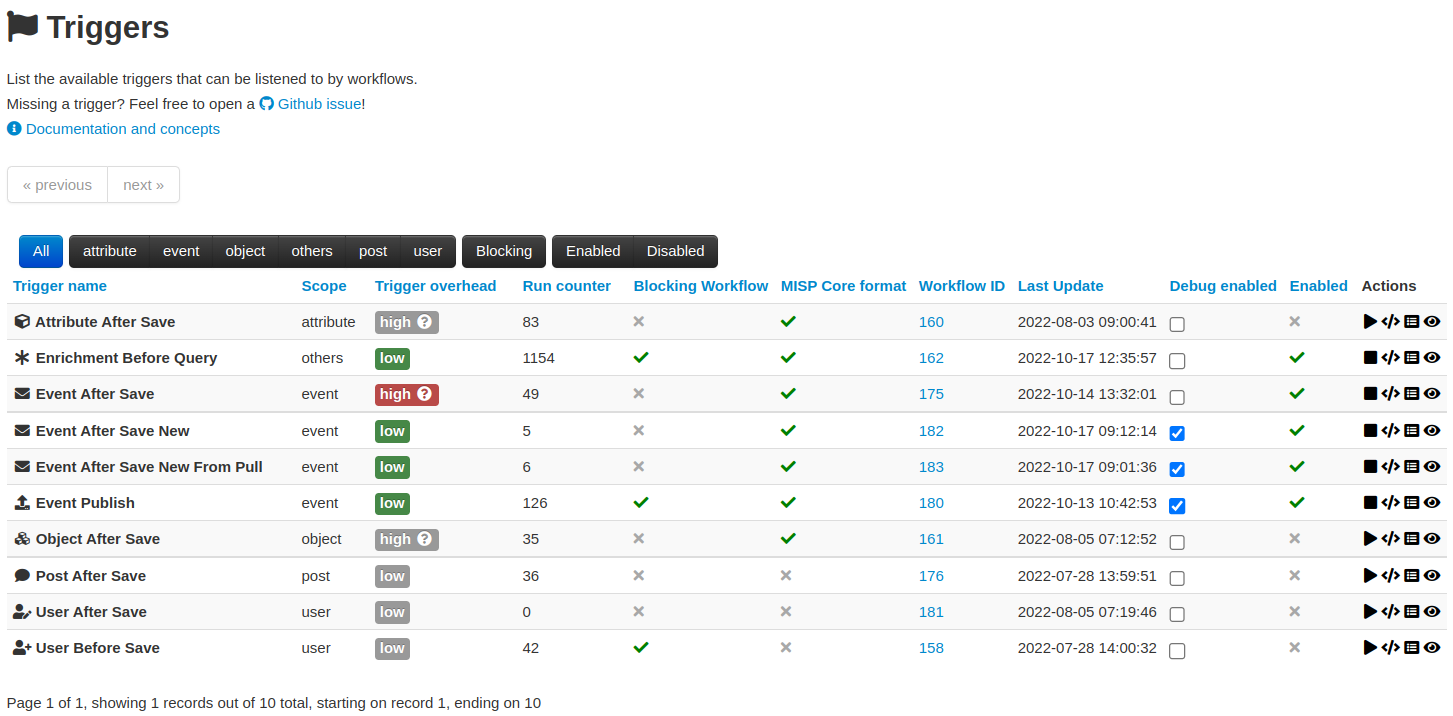
\includegraphics[width=1.0\linewidth]{pictures/triggers.png}
    \end{center}
\end{frame}

\begin{frame}
    \frametitle{What kind of conditions?}
    \vspace*{0.25em}
    
\includegraphics[width=70px]{pictures/sc-condition.png}
    \vspace*{0.25em}
    \begin{itemize}
        \item A MISP Event is tagged with \texttt{tlp:red}
        \item The distribution of an Attribute is a sharing group
        \item The creator organisation is \texttt{circl.lu}
        \item Or any other \textbf{generic} conditions
    \end{itemize}

    \vspace*{0.5em}
    {\Large \faIcon{question-circle}} These are also called \textbf{Logic modules}
    \begin{center}
        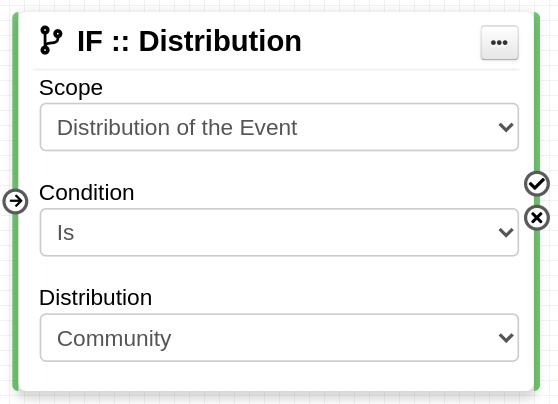
\includegraphics[width=0.43\textwidth]{pictures/logic-module.png}
    \end{center}
\end{frame}

\begin{frame}
    \frametitle{Workflow - Logic modules}
    \begin{itemize}
        \item 
\includegraphics[width=12px]{pictures/sc-condition-icon.png} \textbf{logic} modules: Allow to redirect the execution flow.
        \begin{itemize}
            \item IF conditions
            \item Delay execution
        \end{itemize}
    \end{itemize}
    \begin{center}
        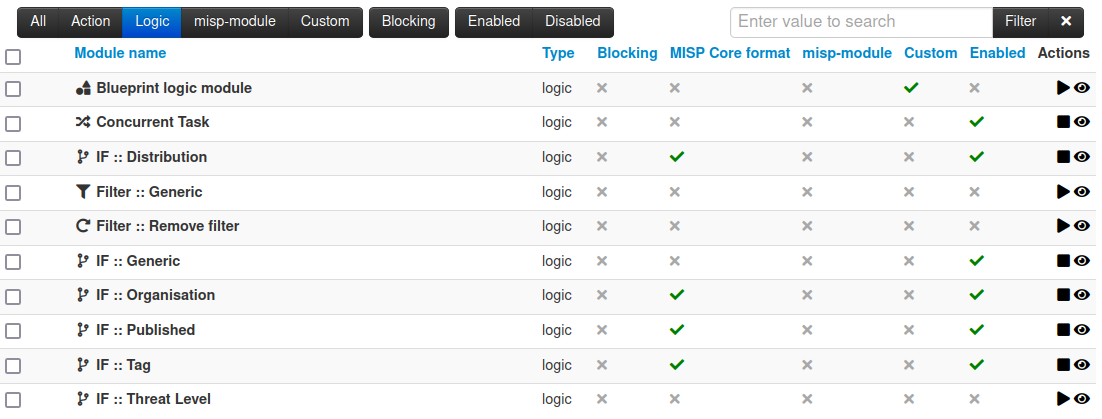
\includegraphics[width=1.0\linewidth]{pictures/logic-module-index.png}
    \end{center}
\end{frame}

\begin{frame}
    \frametitle{What kind of actions?}
    \vspace*{0.25em}
    
\includegraphics[width=60px]{pictures/sc-action.png}
    \vspace*{0.25em}
    \begin{itemize}
        \item Send an email notification
        \item Perform enrichments
        \item Send a chat message on MS Teams
        \item Attach a local tag
        \item ...
    \end{itemize}

    \vspace*{0.5em}
    {\Large \faIcon{question-circle}} These are also called \textbf{Action modules}
    \begin{center}
        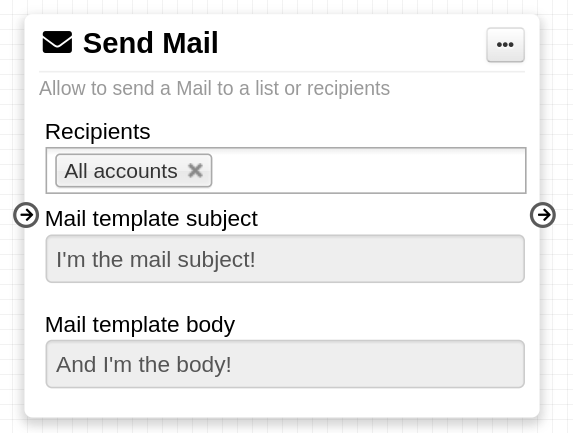
\includegraphics[width=0.43\textwidth]{pictures/action-module.png}
    \end{center}
\end{frame}

\begin{frame}
    \frametitle{Workflow - Action modules}
    \begin{itemize}
        \item 
\includegraphics[width=12px]{pictures/sc-action-icon.png} \textbf{action} modules: Allow to executes operations
        \begin{itemize}
            \item Tag operations
            \item Send notifications
            \item Webhooks \& Custom scripts
        \end{itemize}
    \end{itemize}
    \begin{center}
        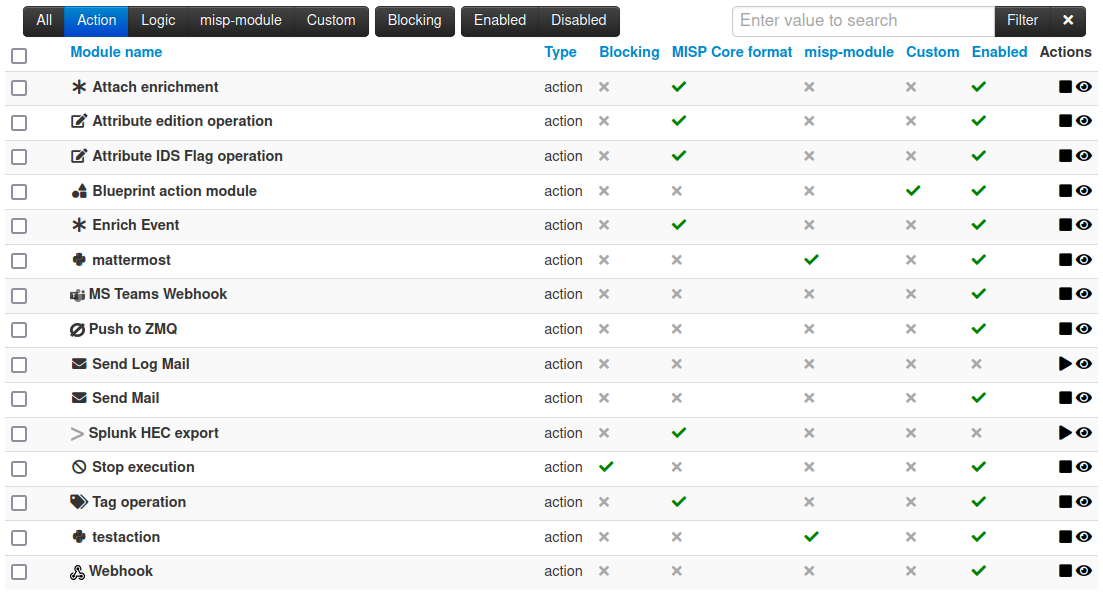
\includegraphics[width=0.95\linewidth]{pictures/action-module-index.png}
    \end{center}
\end{frame}

\begin{frame}
    \frametitle{What is a MISP Workflow?}
    \begin{itemize}
        \item Sequence of all nodes to be executed in a specific order
        \item Workflows can be enabled / disabled
        \item A Workflow is associated to \textbf{1-and-only-1 trigger}
    \end{itemize}
    \vspace*{0.5em}
    \begin{center}
        \frame{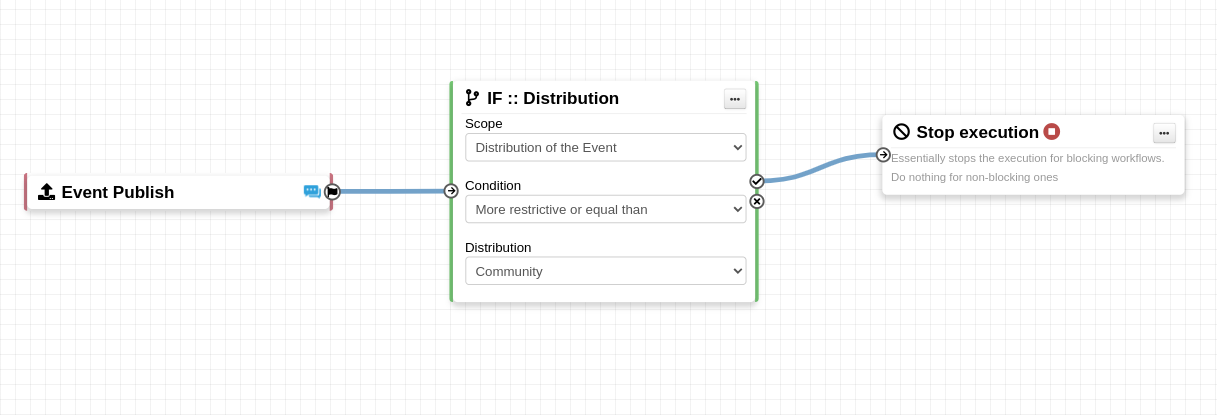
\includegraphics[width=1.0\linewidth]{pictures/simple-workflow.png}}
    \end{center}
\end{frame}

\begin{frame}
    \frametitle{Workflow execution for Event publish}
    \begin{itemize}
        \setlength\itemsep{1em}
        \item[] \hspace*{-2em}
\includegraphics[width=16px]{pictures/sc-event-icon.png} \hspace*{0.25em} An Event is about to be published
        \begin{itemize}
            \item The workflow for the \texttt{event-publish} trigger starts
        \end{itemize}
        \item[] \hspace*{-2em}
\includegraphics[width=16px]{pictures/sc-condition-icon.png} \hspace*{0.25em} Conditions are evaluated
        \begin{itemize}
            \item They might change the path taken during the execution
        \end{itemize}
        \item[] \hspace*{-2em}
\includegraphics[width=16px]{pictures/sc-action-icon.png} \hspace*{0.25em} Actions are executed
        \begin{itemize}
            \setlength\itemsep{0.75em}
            \item {\bf\color{green!50!black}success}: Continue the publishing action
            \hspace*{-4em}
\includegraphics[width=1.0\textwidth]{pictures/log-entry-publish-success.png}
            \item {\bf\color{red}failure} | \texttt{\color{red}blocked}: Stop publishing and log the reason
            \hspace*{-4em}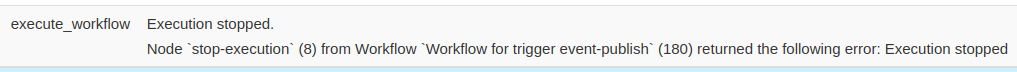
\includegraphics[width=1.0\textwidth]{pictures/log-entry-publish-blocked.png}
        \end{itemize}
    \end{itemize}
\end{frame}

\begin{frame}
    \frametitle{Blocking and non-blocking}
    Two types of workflows:
    \vspace{0.5em}
    \begin{itemize}
        \item[] \hspace*{-2em}
\includegraphics[valign=m,width=48px]{pictures/blocking-workflow.png} Workflows
        \begin{itemize}
            \item Can prevent / block the original event to happen
            \item If a \textbf{blocking module}
\includegraphics[valign=b,width=12px]{pictures/blocking-module.png} blocks the action
        \end{itemize}
        \vspace{0.5em}
        \item[] \hspace*{-2em}
\includegraphics[valign=b,width=56px]{pictures/non-blocking-workflow.png} Workflows execution outcome has no impact
        \begin{itemize}
            \item No way to prevent something that happened in the past
        \end{itemize}
        \begin{center}
            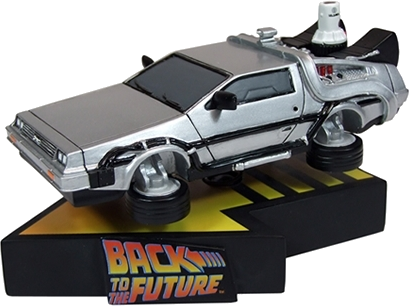
\includegraphics[width=0.3\linewidth]{pictures/time-machine.png}
        \end{center}
    \end{itemize}
\end{frame}

\begin{frame}
    \frametitle{Sources of Workflow modules (0)}
    Currently 36 built-in modules.
    \vspace{1em}
    \begin{itemize}
        \item \textbf{Trigger} module (11): built-in \textbf{only}
        \begin{itemize}
            \item Get in touch if you want more
        \end{itemize}
        \item \textbf{Logic} module (10): built-in \& \textbf{custom}
        \item \textbf{Action} module (15): built-in \& \textbf{custom}
    \end{itemize}
    \vspace*{2.0em}
\end{frame}

\begin{frame}
    \frametitle{Sources of Workflow modules (1)}
    \begin{itemize}
        \item Built-in \textbf{default} modules
        \begin{itemize}
            \item Part of the MISP codebase
            \item Get in touch if you want us to increase the selection (or merge PR!)
        \end{itemize}
    \end{itemize}
    \vspace*{0.5em}
    \begin{center}
        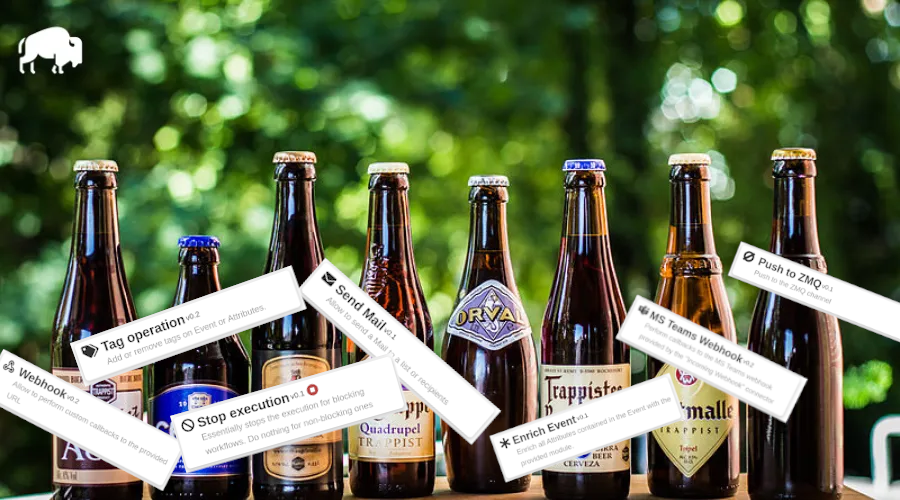
\includegraphics[width=0.8\linewidth]{pictures/module-buffet.png}
    \end{center}
\end{frame}

\begin{frame}
    \frametitle{Sources of Workflow modules (2)}
    User-defined \textbf{custom} modules
    \vspace*{0.5em}
    \begin{columns}
        \begin{column}{0.5\textwidth}
            \begin{itemize}
                \item Written in PHP
                \item Extend existing modules
                \item MISP code reuse
            \end{itemize}
        \end{column}
        \begin{column}{0.5\textwidth}
            
\includegraphics[width=1.0\linewidth]{pictures/php-joke.jpg}
        \end{column}
    \end{columns}
\end{frame}

\begin{frame}
    \frametitle{Sources of Workflow modules (3)}
    Modules from the 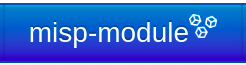
\includegraphics[width=0.20\linewidth]{pictures/misp-module-icon.png} \textbf{enrichment service}
    \vspace*{0.5em}
    \begin{columns}
        \begin{column}{0.50\textwidth}
            \begin{itemize}
                \item Written in Python
                \item Can use any python libraries
                \item Plug \& Play
            \end{itemize}
        \end{column}
        \begin{column}{0.50\textwidth}
            
\includegraphics[width=1.0\linewidth]{pictures/python-joke.png}
        \end{column}
    \end{columns}
\end{frame}

\begin{frame}
    \frametitle{Demo by examples}
    \begin{enumerate}
        \item[WF-1.] Send an email to \textbf{all} when a new event has been pulled
        \vspace*{2em}
        \item[WF-2.] Block queries on 3rd party services when \textbf{tlp:red} or \textbf{PAP:red}
        \begin{itemize}
            \item \textbf{tlp:red}: For the eyes and ears of individual recipients only
            \item \textbf{PAP:RED}: Only passive actions that are not detectable from the outside
        \end{itemize}
    \end{enumerate}
\end{frame}

% \section{Workflow - Getting started}
\begin{frame}
    \frametitle{
        \huge
        \linebreak
        \linebreak
        \linebreak
        Workflow - Getting started
        \vspace{1em}
    }
    \textbf{Objective:} How to install \& configure workflows
    \begin{center}
        
\includegraphics[width=0.2\linewidth]{pictures/getting-started}
    \end{center}
\end{frame}

\begin{frame}
    \frametitle{Getting started with workflows (1)}
    \begin{center}
        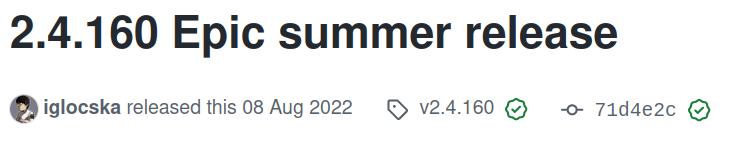
\includegraphics[width=0.9\linewidth]{pictures/workflow-release.png}
    \end{center}
    \begin{enumerate}
        \item Update your MISP server
        \item Update all your sub-modules
    \end{enumerate}
    \begin{center}
        
\includegraphics[width=0.6\textwidth]{pictures/upgrade-people.jpeg}
    \end{center}
\end{frame}

\begin{frame}
    \frametitle{Getting started with workflows (2)}
    Review MISP settings:
    \begin{enumerate}
        \item Make sure \texttt{MISP.background\_jobs} is turned on
        \item Make sure workers are up-and-running and healthy
        \item Turn the setting \texttt{Plugin.Workflow\_enable} on
    \end{enumerate}
    \begin{center}
        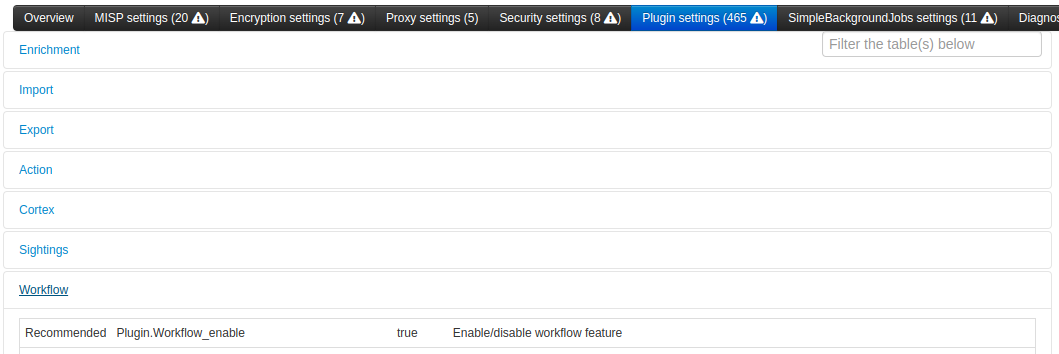
\includegraphics[width=1.0\linewidth]{pictures/settings-2.png}
    \end{center}
\end{frame}

\begin{frame}
    \frametitle{Getting started with workflows (3)}
    Review MISP settings:
    \begin{enumerate}
        \setcounter{enumi}{3}
        \item {[optional:misp-module]} Turn the setting \texttt{Plugin.Action\_services\_enable} on
    \end{enumerate}
    \begin{center}
        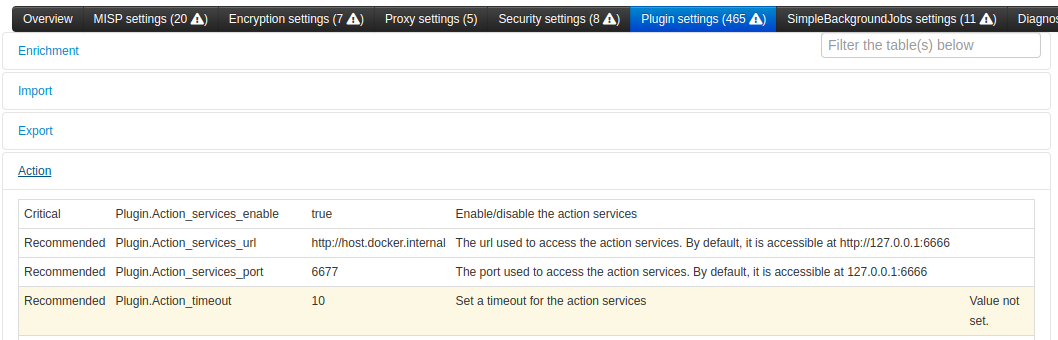
\includegraphics[width=1.0\linewidth]{pictures/settings-1.png}
    \end{center}
\end{frame}

\begin{frame}[fragile]
    \frametitle{Getting started with workflows (4)}
    If you wish to use action modules from \texttt{misp-module}, make sure to have:
    \begin{itemize}
        \item The latest update of \texttt{misp-module}
        \begin{itemize}
            \item There should be an \texttt{action\_mod} module type in \url{misp-modules/misp\_modules/modules}
        \end{itemize}
        \item Restarted your \texttt{misp-module} application
    \end{itemize}
    \vspace{1em}
    \begin{lstlisting}[language=text,firstnumber=1]
# This command should show all `action` modules
$ curl -s http://127.0.0.1:6666/modules | \
jq '.[] | select(.meta."module-type"[] | contains("action")) | 
{name: .name, version: .meta.version}'
    \end{lstlisting}
\end{frame}

\begin{frame}
    \frametitle{Getting started with workflows (5)}
    \centering
    {\Large Everything is ready?}\\
    \vspace*{3em}
    {\LARGE Let's see how to build a workflow!}
    \begin{center}
        
\includegraphics[width=24px]{pictures/build-icon.png}
    \end{center}
\end{frame}

\begin{frame}
    \frametitle{Creating a workflow with the editor}
    \begin{enumerate}
        \item Prevent event publication if \textbf{tlp:red} tag
        \item Send a mail to \texttt{admin@admin.test} about potential data leak
        \item Otherwise, send a notification on Mattermost
    \end{enumerate}
\end{frame}

% \section{Considerations when working with workflows}
\begin{frame}
    \frametitle{
        \huge
        \linebreak
        \linebreak
        \linebreak
        Considerations when working with workflows
        \vspace{1em}
    }
    \textbf{Objective:} Overview of some common pitfalls
    \begin{center}
        
\includegraphics[width=24px]{pictures/radar.png}
    \end{center}
\end{frame}

\begin{frame}
    \frametitle{Working with the editor - Operations not allowed}
    Execution loop are not authorized
    \vspace*{1em}
    \begin{columns}
        \begin{column}{0.7\textwidth}
            \frame{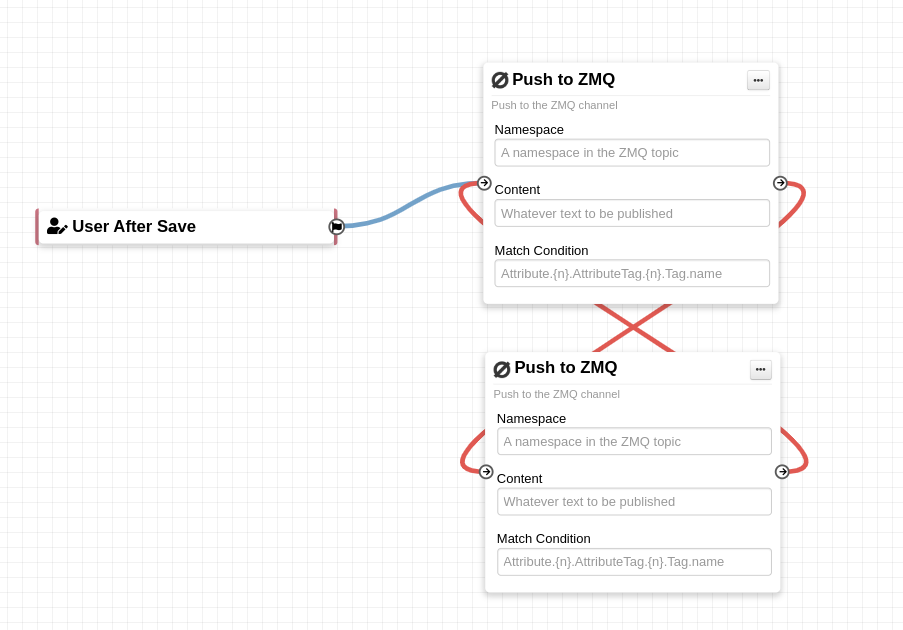
\includegraphics[width=1.0\linewidth]{pictures/editor-not-allowed-1.png}}
        \end{column}
        \begin{column}{0.3\textwidth}
            \frame{
\includegraphics[width=1.0\linewidth]{pictures/infinite-loop.jpg}}
        \end{column}
    \end{columns}
\end{frame}

\begin{frame}
    \frametitle{Recursive workflows}
    \frame{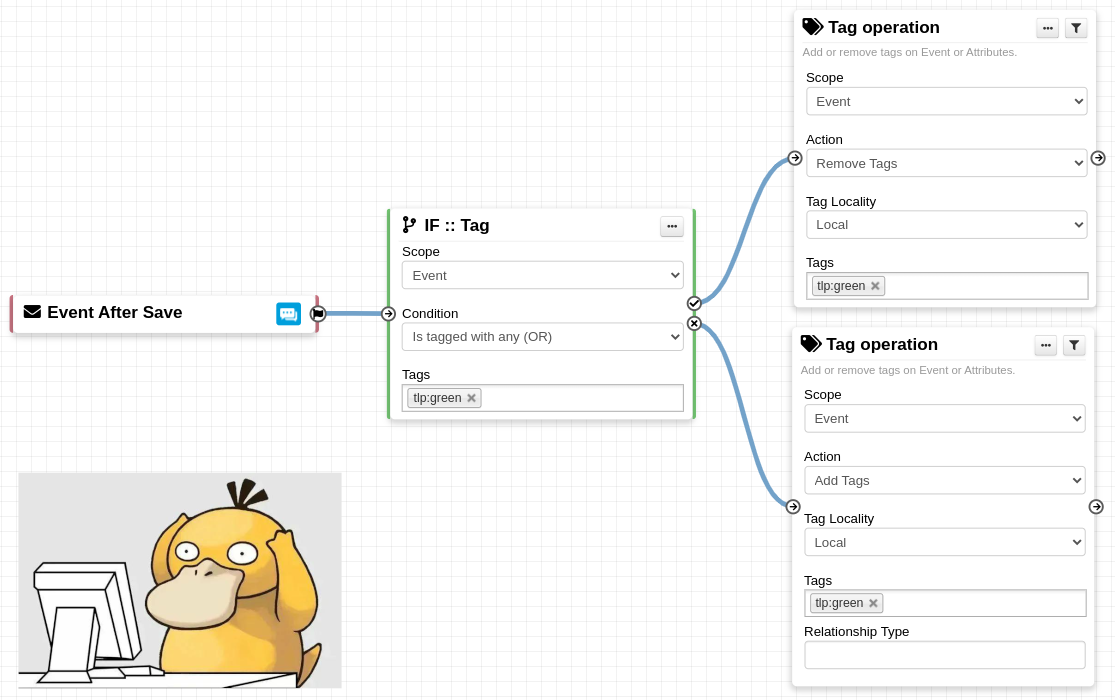
\includegraphics[width=1.0\linewidth]{pictures/recursive-workflow.png}}
    \danger Recursion: If an action re-run the workflow
\end{frame}

\begin{frame}
    \frametitle{Working with the editor - Operations not allowed}
    Multiple connections from the same output
    \vspace*{1em}
    \begin{columns}
        \begin{column}{0.7\textwidth}
            \frame{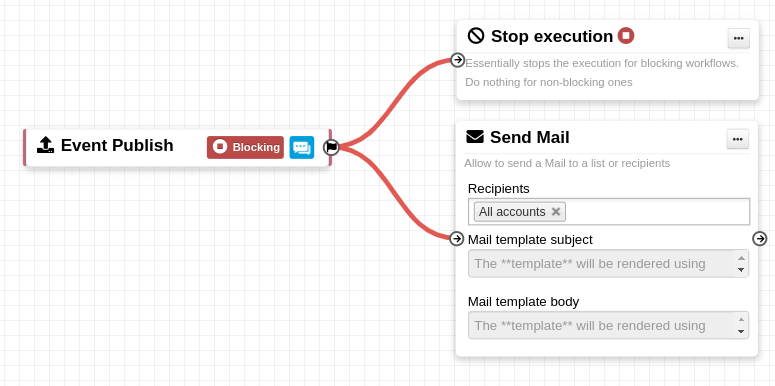
\includegraphics[width=1.0\linewidth]{pictures/editor-not-allowed-2.png}}
        \end{column}
        \begin{column}{0.3\textwidth}
            \frame{
\includegraphics[width=1.0\linewidth]{pictures/two-paths.jpeg}}
        \end{column}
    \end{columns}
    \begin{itemize}
        \item Execution order not guaranted
        \item Confusing for users
    \end{itemize}
\end{frame}

\begin{frame}
    \frametitle{Working with the editor}
    Cases showing a warning:
    \begin{itemize}
        \item \textbf{Blocking} modules 
\includegraphics[width=10px]{pictures/blocking-module.png} in a 
\includegraphics[valign=b,width=56px]{pictures/non-blocking-workflow.png} workflow 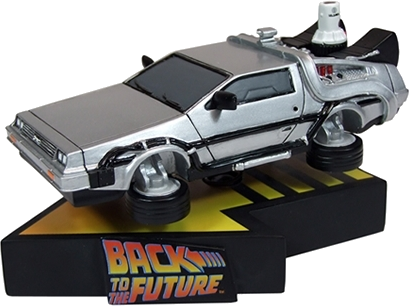
\includegraphics[width=0.12\linewidth]{pictures/time-machine.png}
        \item \textbf{Blocking} modules 
\includegraphics[width=10px]{pictures/blocking-module.png} after a \textbf{concurrent tasks} module
        \begin{center}
            \frame{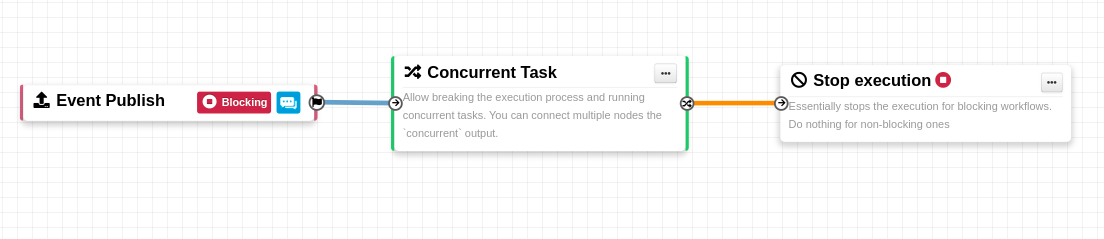
\includegraphics[width=1.0\linewidth]{pictures/editor-warning-1.png}}
        \end{center}
    \end{itemize}
\end{frame}

% \section{Advanced usage}
\begin{frame}
    \frametitle{
        \huge
        \linebreak
        \linebreak
        \linebreak
        Advanced usage
        \vspace{1em}
    }
    \textbf{Objective:} Overview of Blueprints, Data format and Filtering
\end{frame}

\begin{frame}
    \frametitle{Workflow blueprints}
    \hspace*{0.9\textwidth}\includegraphics[width=32px]{pictures/blueprint-32.png}
    \vspace*{-2em}
    \begin{enumerate}
        \item Blueprints allow to \textbf{re-use parts} of a workflow in another one
        \item Blueprints can be saved, exported and \textbf{shared}
    \end{enumerate}
    \begin{center}
        \includegraphics[width=0.5\linewidth]{pictures/blueprint-debugging.png}
    \end{center}
    Blueprints sources:
    \begin{enumerate}
        \item Created or imported by users
        \item From the \texttt{MISP/misp-workflow-blueprints} repository\footnote{\scriptsize https://github.com/MISP/misp-workflow-blueprints}
    \end{enumerate}
\end{frame}

\begin{frame}
    \frametitle{Logic module: Concurrent Task}
    \begin{itemize}
        \item Logic module allowing \textbf{multiple output} connections
        \item \textbf{Postpone the execution} for remaining modules
        \item Convert \includegraphics[valign=b,width=44px]{pictures/blocking-workflow.png} \faIcon{long-arrow-alt-right} \includegraphics[valign=b,width=56px]{pictures/non-blocking-workflow.png}
    \end{itemize}
    \begin{center}
        \frame{\includegraphics[width=0.5\linewidth]{pictures/module-concurrent.png}}
    \end{center}
\end{frame}

\begin{frame}
    \frametitle{Data format in Workflows}
    \begin{center}
        \includegraphics[width=0.7\linewidth]{pictures/workflow-trigger.png}
    \end{center}
    \begin{itemize}
        \item In most cases, the format is the \textbf{MISP Core format}
        \begin{itemize}
            \item Attributes are \textbf{always encapsulated} in the Event or Object
        \end{itemize}
        \item But has \textbf{additional properties}
        \begin{itemize}
            \item Additional key \textbf{\texttt{\_AttributeFlattened}}
            \item Additional key \textbf{\texttt{\_allTags}}
            \item Additional key \textbf{\texttt{inherited}} for Tags
        \end{itemize}
    \end{itemize}
\end{frame}

\begin{frame}[fragile]
    \frametitle{Hash path filtering (1)}
    Filtering and checking conditions using hash path expression.
    \begin{lstlisting}[language=javascript,firstnumber=1]
    $path_expression = '{n}[name=fred].id';
    $users = [
        {'id': 123, 'name': 'fred', 'surname': 'bloggs'},
        {'id': 245, 'name': 'fred', 'surname': 'smith'},
        {'id': 356, 'name': 'joe', 'surname': 'smith'},
    ];
    $ids = Hash::extract($users, $path_expression);
    // => $ids will be [123, 245]
    \end{lstlisting}
    \begin{columns}
        \begin{column}{0.6\textwidth}
            \begin{center}
                \includegraphics[width=0.7\linewidth]{pictures/attribute-json.png}
            \end{center}
        \end{column}
        \begin{column}{0.4\textwidth}
            \includegraphics[width=1.0\linewidth]{pictures/module-if-generic.png}
        \end{column}
    \end{columns}
\end{frame}

\begin{frame}[fragile]
    \frametitle{Hash path filtering (2)}
    Hash path filtering can be used to \textbf{filter} data \textbf{on the node} it is passed to or on the \textbf{execution path}.
    \begin{center}
        \includegraphics[width=0.58\linewidth]{pictures/node-filtering.png}
        \includegraphics[width=0.4\linewidth]{pictures/node-generic-filter.png}
    \end{center}
\end{frame}

\begin{frame}[fragile]
    \frametitle{Hash path filtering - Example}

\begin{lstlisting}[language=javascript,firstnumber=1]
{
    "Event": {
        "uuid": ...
        "timestamp": ...
        "distribution": 1,
        "published": false,
        "Attribute": [
            {
                "type": "ip-src",
                "value": "8.8.8.8", ...
            },
            {
                "type": "domain",
                "value": "misp-project.org", ...
            }
        ],
        ...
    }
}
\end{lstlisting}
    \begin{enumerate}
        \item Access Event distribution
        \begin{itemize}
            \item \texttt{Event.distribution}
        \end{itemize}
    \end{enumerate}
\end{frame}

\begin{frame}[fragile]
    \frametitle{Hash path filtering - Exercise (1)}

\begin{lstlisting}[language=javascript,firstnumber=1]
{
    "Event": {
        "uuid": ...
        "distribution": 1,
        "published": false,
        "Attribute": [
            {
                "type": "ip-src",
                "value": "8.8.8.8", ...
            },
            {
                "type": "domain",
                "value": "misp-project.org", ...
            }
        ],
        ...
    }
}
\end{lstlisting}
    \begin{enumerate}
        \setcounter{enumi}{1}
        \item Access Event published state
        \pause
        \begin{itemize}
            \item \texttt{Event.published}
        \end{itemize}
    \end{enumerate}
\end{frame}

\begin{frame}[fragile]
    \frametitle{Hash path filtering - Exercise (2)}

\begin{lstlisting}[language=javascript,firstnumber=1]
{
    "Event": {
        "uuid": ...
        "distribution": 1,
        "published": false,
        "Attribute": [
            {
                "type": "ip-src",
                "value": "8.8.8.8", ...
            },
            {
                "type": "domain",
                "value": "misp-project.org", ...
            }
        ],
        ...
    }
}
\end{lstlisting}
    \begin{enumerate}
        \setcounter{enumi}{2}
        \item Access all Attribute types
        \begin{itemize}
            \item Hint: Use \texttt{\bf \{n\}} to loop 
            \pause
            \item \texttt{Event.Attribute.\{n\}.type}
        \end{itemize}
    \end{enumerate}
\end{frame}

\begin{frame}[fragile]
    \frametitle{Hash path filtering - Exercise (3)}

\begin{lstlisting}[language=javascript,firstnumber=1]
{
    "Event": {
        "Attribute": [
            {
                "type": "ip-src",
                "value": "8.8.8.8",
                "Tag": [
                    {
                        "name": "PAP:AMBER", ...
                    }
                ], ...
            }
        ],
        ...
    }
}
\end{lstlisting}
    \begin{enumerate}
        \setcounter{enumi}{2}
        \item Access all Tags attached to Attributes
        \pause
        \begin{itemize}
            \item \texttt{Event.Attribute.\{n\}.Tag.\{n\}.name}
        \end{itemize}
    \end{enumerate}
\end{frame}

\begin{frame}[fragile]
    \frametitle{Hash path filtering - Exercise (4)}

\begin{lstlisting}[language=javascript,firstnumber=1]
{
    "Event": {
        "Tag": [
            {
                "name": "tlp:green", ...
            }
        ], ...
        "Attribute": [
            {
                "value": "8.8.8.8",
                "Tag": [
                    {
                        "name": "PAP:AMBER", ...
                    }
                ], ...
            }
        ],
    }
}
\end{lstlisting}
    \begin{enumerate}
        \setcounter{enumi}{3}
        \item Access all Tags attached to Attributes and from the Event
        \pause
        \begin{itemize}
            \item \texttt{Event.Attribute.\{n\}.\_allTags.\{n\}.name}
        \end{itemize}
    \end{enumerate}
\end{frame}

\begin{frame}[fragile]
    \frametitle{Hash path filtering - Exercise (4)}

\begin{lstlisting}[language=javascript,firstnumber=1]
{
    "Event": {
        "Tag": [...],
        "Attribute": [
            {
                "value": "8.8.8.8",
                "_allTags": [
                    {
                        "name": "tlp:green",
                        "inherited": true, ...
                    },
                    {
                        "name": "PAP:AMBER",
                        "inherited": false, ...
                    }
                ],
            }
        ...
}
\end{lstlisting}
    \begin{enumerate}
        \setcounter{enumi}{3}
        \item Access all Tags attached to Attributes and from the Event
        \begin{itemize}
            \item \texttt{Event.Attribute.\{n\}.\_allTags.\{n\}.name}
        \end{itemize}
    \end{enumerate}
\end{frame}


\begin{frame}
    \frametitle{Fitlering data on which to apply a module}
    What happens when an Event is about to be published?
    \begin{center}
        \includegraphics[width=1.0\textwidth]{pictures/remove-ids-1.png}
    \end{center}
    \pause
    \vspace{1em}
    All Attributes get their \texttt{to\_ids} turned off.\\
    \vspace{1em}
    How could we force that action only on Attribute of type \texttt{comment}?
    \begin{center}
        $\rightarrow$ Hash path filtering!
    \end{center}
\end{frame}

\begin{frame}
    \frametitle{Fitlering data on which to apply a module}
    \begin{center}
        \includegraphics[width=0.5\textwidth]{pictures/remove-ids-3.png}
    \end{center}
    \begin{center}
        \includegraphics[width=0.9\textwidth]{pictures/remove-ids-2.png}
    \end{center}
\end{frame}

\begin{frame}
    \frametitle{Fitlering data on which to apply on multiple modules}
    New feature as of \textbf{v2.4.171} allows setting filters on a path.
    \begin{center}
        \includegraphics[width=1.0\textwidth]{pictures/remove-ids-generic.png}
    \end{center}
\end{frame}

\section{Exercices}
\begin{frame}
    \frametitle{Exercises}
    \begin{enumerate}
        \item PAP:RED and tlp:red blocking
        \item Replace tlp:white by tlp:clear
        \item Attach tag on attribute having a low value (<50) in bgp ranking
        \item Remove to\_ids flag for attribute having a match in hashlookup
    \end{enumerate}
\end{frame}

\section{Debugging}
\begin{frame}
    \frametitle{Debugging Workflows: Log Entries}
    \begin{itemize}
        \item Workflow execution is logged in the application logs:
        \begin{itemize}
            \item \texttt{/admin/logs/index}
            \item Note: Might be phased out as its too verbose
        \end{itemize}
        \item Or stored on disk in the following file:
        \begin{itemize}
            \item \texttt{/app/tmp/logs/workflow-execution.log}
        \end{itemize}
    \end{itemize}
    \begin{center}
        \includegraphics[width=1.0\linewidth]{pictures/workflow-debug.png}
    \end{center}
\end{frame}

\begin{frame}
    \frametitle{Debugging Workflows: Debug mode}
    \begin{itemize}
        \item The \includegraphics[width=70px]{pictures/debug-mode.png} can be turned on for each workflows
        \item Each nodes will send data to the provided URL
        \begin{itemize}
            \item Configure the setting: \texttt{Plugin.Workflow\_debug\_url}
        \end{itemize}
        \item Result can be visualized in
        \begin{itemize}
            \item \textbf{offline}: \texttt{tools/misp-workflows/webhook-listener.py}
            \item \textbf{online}: \url{requestbin.com} or similar websites
        \end{itemize}
    \end{itemize}
    \begin{center}
        \includegraphics[width=0.6\linewidth]{pictures/request-bin.png}
    \end{center}
\end{frame}

\begin{frame}
    \frametitle{Debugging modules: Stateless execution}
    \begin{itemize}
        \item Test custom modules with custom input
    \end{itemize}
    \begin{center}
        \includegraphics[width=1.0\linewidth]{pictures/stateless-execution.png}
    \end{center}
\end{frame}

\begin{frame}
    \frametitle{Debugging modules: Re-running workflows}
    \begin{itemize}
        \item Try workflows with custom input
        \item Re-run workflows to ease debugging
    \end{itemize}
    \begin{center}
        \frame{\includegraphics[width=0.55\linewidth]{pictures/running-workflows.png}}
    \end{center}
\end{frame}

\begin{frame}
    \frametitle{Debugging options}
    \begin{columns}
        \begin{column}{0.6\textwidth}
            \begin{itemize}
                \item Workflow \textbf{execution and outcome}
                \item Module \textbf{execution and outcome}
                \item \textbf{Live} workflow debugging with module inspection
                \item \textbf{Re-running/testing} workflows with custom data
                \item \textbf{Stateless} module execution
            \end{itemize}
        \end{column}
        \begin{column}{0.4\textwidth}
            \includegraphics[width=1.0\linewidth]{pictures/enough-debugging.jpg}
        \end{column}
    \end{columns}
\end{frame}

% \section{Extending the system}
\begin{frame}
    \frametitle{
        \huge
        \linebreak
        \linebreak
        \linebreak
        Extending the system
        \vspace{1em}
    }
    \begin{center}
        \includegraphics[width=0.6\linewidth]{pictures/craft.jpg}
    \end{center}
\end{frame}

\begin{frame}
    \frametitle{Creating a new module in PHP}
    \begin{center}
        \includegraphics[scale=0.1]{pictures/PHP-logo.png}
    \end{center}
    \vspace*{2em}
    \begin{itemize}
        \item \texttt{\small \textbf{app/Lib/}WorkflowModules/action/[module\_name].php}
        \item Designed to be easilty extended
        \begin{itemize}
            \item Helper functions
            \item Module configuration as variables
            \item Implement runtime logic
        \end{itemize}
        \item Main benefits
        \begin{itemize}
            \item Fast
            \item Re-use existing functionalities
            \item No need for misp-modules
        \end{itemize}
    \end{itemize}
\end{frame}

\begin{frame}
    \frametitle{Creating a new module in PHP}
    \begin{center}
        \includegraphics[width=1.0\linewidth]{pictures/custom-1.png}
    \end{center}
\end{frame}

\begin{frame}
    \frametitle{Creating a new module in Python}
    \begin{center}
        \includegraphics[scale=0.05]{pictures/python-logo.png}
    \end{center}
    \begin{itemize}
        \item Similar to how other \texttt{misp-modules} are implemented
        \begin{itemize}
            \item Helper functions
            \item Module configuration as variables
            \item Implement runtime logic
        \end{itemize}
        \item Main benefits
        \begin{itemize}
            \item Easier than PHP
            \item Lots of libraries for integration
        \end{itemize}
    \end{itemize}
\end{frame}

\begin{frame}
    \frametitle{Creating a new module in Python}
    \begin{center}
        \includegraphics[width=1.0\linewidth]{pictures/custom-2.png}
    \end{center}
\end{frame}

\begin{frame}
    \frametitle{Should I migrate to MISP Workflows}
    I have automation in place using the API / ZMQ. Should I move to Workflows?
    \vspace{1em}
    \begin{itemize}
        \item I (have/am planning to create) a curation pipeline using the API, should I port them to workflows?
        \begin{itemize}
            \item \textbf{No} in general, but WF can be used to start the curation process
        \end{itemize}
        \item What if I want to \textbf{block} some actions
        \begin{itemize}
            \item Put the blocking logic in the WF, the remaining outside
        \end{itemize}
        \item Currently, workflows with \textbf{ lots of node are not encouraged}
        \item Bottom line is \textbf{Keep it simple}
    \end{itemize}
\end{frame}

\begin{frame}
    \frametitle{More ideas}
    \begin{itemize}
        \item Notification when new users join an instance
        \item Extend existing MISP behavior: Push correlation in another system
        \item Sanity check to block publishing
        \item Automated alerts for high-priority IOCs
        \item Assign tasks and notify incident response team members
        \item ...
    \end{itemize}
\end{frame}

\begin{frame}
    \frametitle{Future works}
    \begin{columns}
        \begin{column}{0.55\textwidth}
            \begin{itemize}
                \item More \includegraphics[width=12px]{pictures/sc-action-icon.png} modules
                \item More \includegraphics[width=12px]{pictures/sc-condition-icon.png} modules
                \item More \includegraphics[width=12px]{pictures/sc-event-icon.png} triggers
                \item More documentation
                \item Recursion prevention system
                \item On-the-fly data override?
            \end{itemize}
        \end{column}
        \begin{column}{0.45\textwidth}
            \includegraphics[width=1.0\linewidth]{pictures/future-works.jpeg}
        \end{column}
    \end{columns}
\end{frame}

\begin{frame}
    \frametitle{Final words}
    \begin{columns}
        \begin{column}{0.6\textwidth}
            \begin{itemize}
                \item Designed to \textbf{quickly} and \textbf{cheaply} integrate MISP in CTI pipelines
                \item \underline{\textbf{Beta}} Feature unlikely to change. But still..
                \item Waiting for feedback!
                \begin{itemize}
                    \item New triggers?
                    \item New modules?
                    \item What's acheivable
                \end{itemize}
            \end{itemize}
        \end{column}
        \begin{column}{0.4\textwidth}
            \includegraphics[width=1.0\linewidth]{pictures/feeling-of-power.jpg}
        \end{column}
    \end{columns}
    \vspace*{0.5em}
\end{frame}

